\section{Cálculo de Pi.}

Para este ejercicio partimos del fichero \texttt{pi.c} que se nos proporciona. Decidimos
implementar lo que se nos pide (número de iteraciones y media) directamente en el fichero
.c para atajar lo que se nos pide lo más eficientemente posible. Seguimos los siguientes pasos.

\begin{enumerate}
    \item Añade la medición de tiempo para cada algoritmo.
    \item Haz que el tiempo que se indica que ha tardado sea la media de 5 ejecuciones.
    \item Permite incrementar el número de iteraciones hasta el máximo entero dando n pasos.
\end{enumerate}

Podemos ver en la Figura 1.1 el gráfico que obtenemos con los tiempos de ejecución. El tiempo de ejecución
para el método por rectángulos es significativamente superior que para el Leibniz. Esto se puede deber a que:
\begin{enumerate}
    \item El método por rectángulos necesita un mayor número de operaciones matemáticas costosas.
    \item La segunda línea del bucle condicional en el método por rectángulos depende en la primera línea. Esto no ocurre para el de Leibniz.
\end{enumerate}

\begin{figure}[ht]
    \centering
    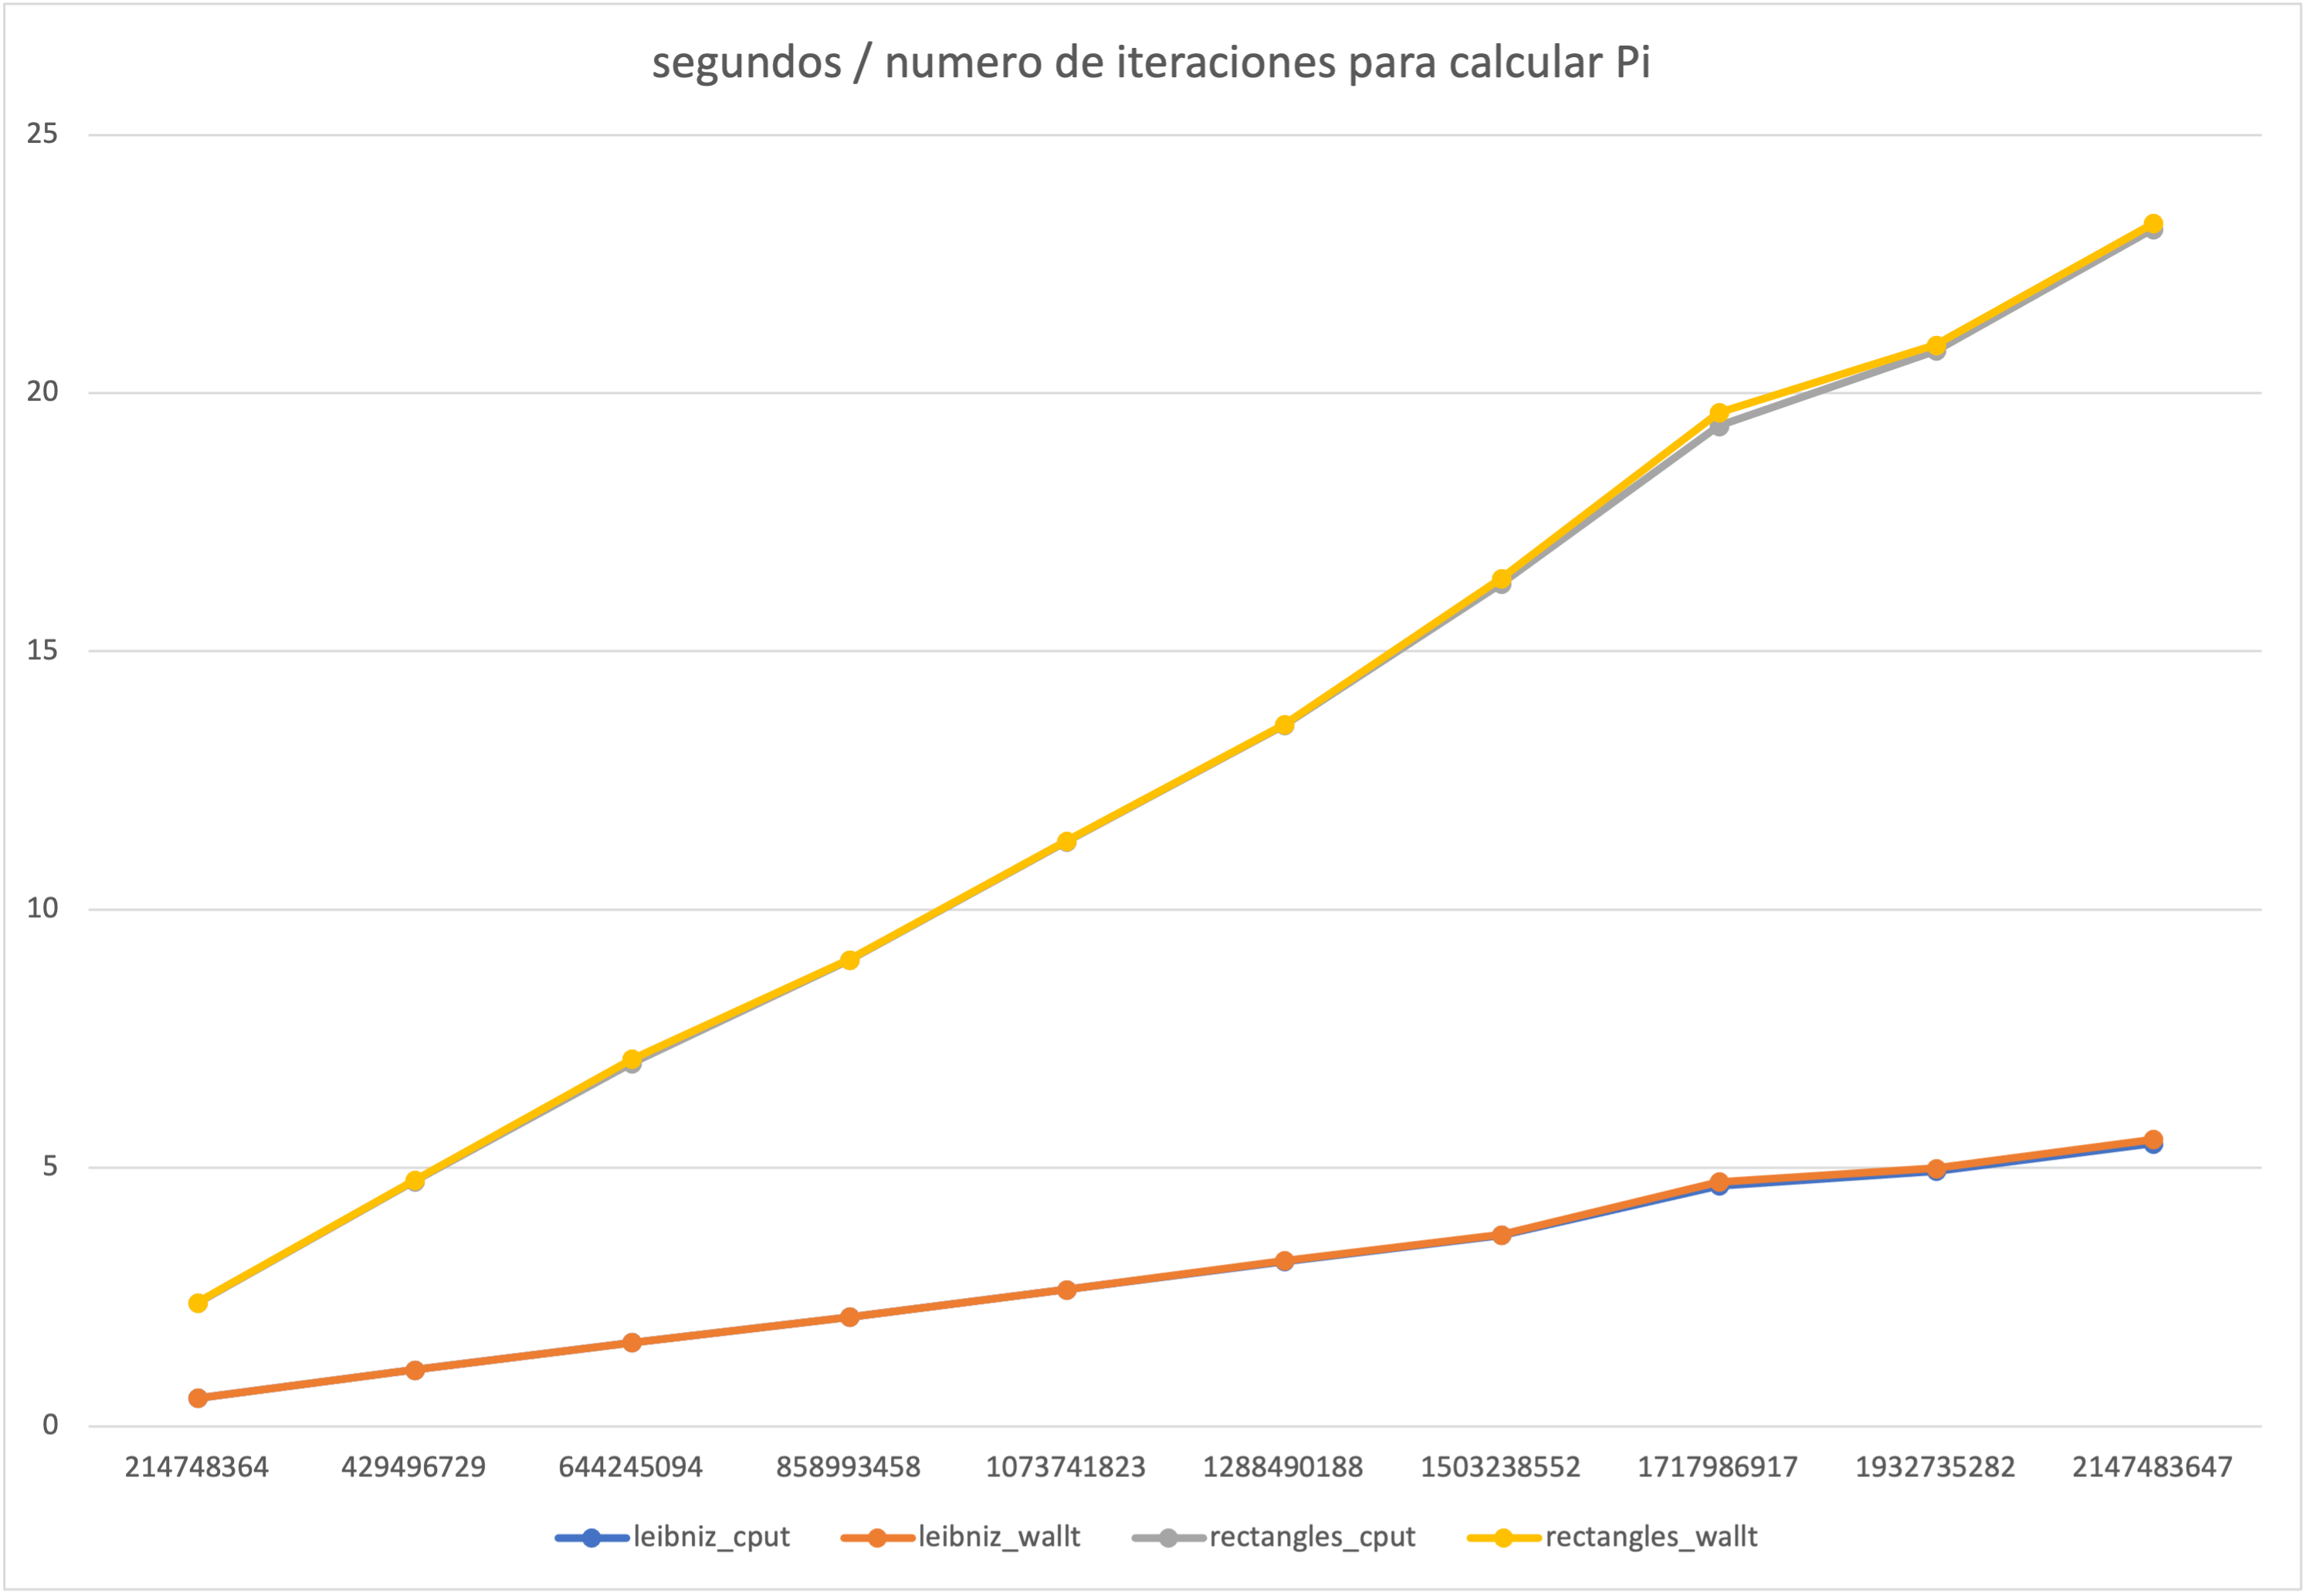
\includegraphics[width=\textwidth]{ej2.png}
    \caption{Relación segundos / número de iteraciones en diez pasos. Podemos observar cómo el
    tiempo de ejecución es lineal según nos desplazamos en el eje de abscisas, siendo ligeramente
    superior el tiempo real transcurrido que el tiempo en que el algoritmo se ejecutaba. Lo primero
    se debe a que ambos algoritmos para el cálculo de Pi tienen un orden de eficiencia $\Theta (n)$.
    Lo segundo se debe a que el algoritmo no tiene que realizar llamadas externas que puedan causar \textit{overhead} y que el ordenador en que se han ejecutado
    los algoritmos apena tiene carga. }
\end{figure}